\begin{figure}[t!]
\centering
\vspace*{-1ex}
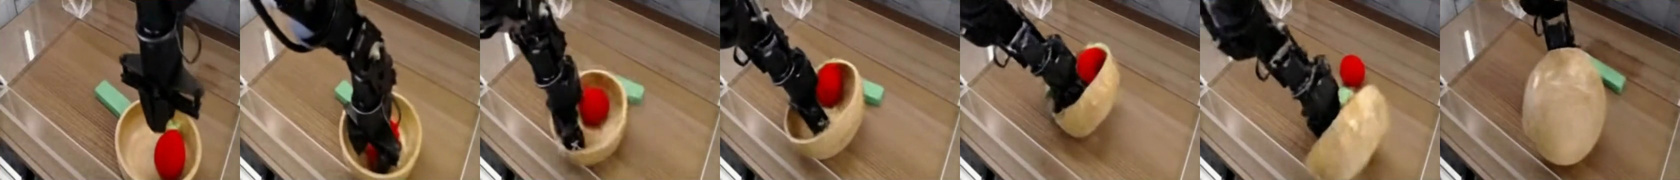
\includegraphics[width=\linewidth]{figures/robotics/soar1} \\[1ex]
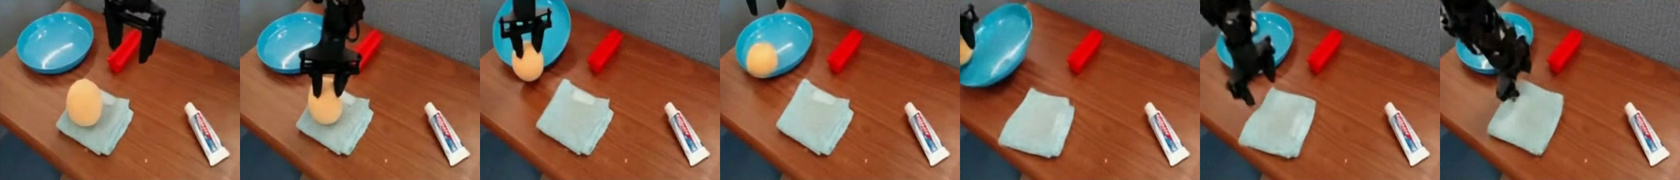
\includegraphics[width=\linewidth]{figures/robotics/soar2} \\[1ex]
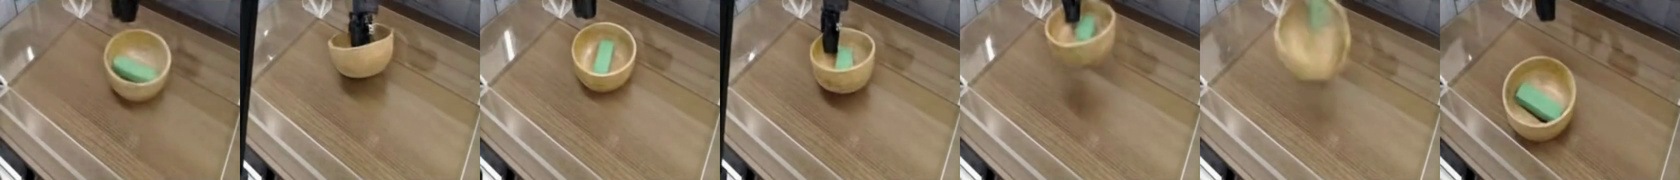
\includegraphics[width=\linewidth]{figures/robotics/soar3}
\caption{机器人反事实行为生成。\method 学习精确的实时模拟环境，使人类操作者能够控制想象中的机器人完成取物、翻转碗、将球推到盘子上、移动毛巾以及投掷碗等操作。}
\label{fig:robotics}
\end{figure}
